

\documentclass[12pt]{article}
\usepackage[margin=1in]{geometry}
\setlength{\emergencystretch}{1em}
\usepackage{amsmath, amssymb, amsthm}
\usepackage{graphicx}
\usepackage{xcolor}
\usepackage{listings}
\usepackage{caption}
\usepackage{natbib}
\usepackage{xr}
\usepackage[hidelinks]{hyperref}
\usepackage{placeins}
\usepackage{float}
\usepackage{pdflscape}
\usepackage{booktabs}
\usepackage{algorithm}
\usepackage{algpseudocode}
\usepackage{subcaption}
\usepackage{multirow}
\usepackage{tikz}
\usetikzlibrary{arrows.meta, positioning}
\DeclareMathOperator{\Var}{Var}
\DeclareMathOperator{\Cov}{Cov}
\newcommand{\E}{\mathbb{E}}
\newcommand\independent{\protect\mathpalette{\protect\independenT}{\perp}}
\def\independenT#1#2{\mathrel{\rlap{$#1#2$}\mkern2mu{#1#2}}}

% ---- switches ---------------------------------------------------------------
\newif\iffixnotes  \fixnotesfalse    % \fixnotesfalse -> clean submission build

\newcommand{\FIX}[2]{%
  \iffixnotes
    \par\smallskip\noindent
    \fcolorbox{orange!50}{orange!7}{%
      \parbox{0.95\linewidth}{\footnotesize\sffamily\color{orange!35!black}%
        \textbf{[#1]\ }#2}}%
    \par\smallskip
  \fi}

\externaldocument[][nocite]{methodology-8.3.5-supplement}

% Changed text is blue when compiled through the highlighted review wrapper.
\definecolor{revisionblue}{RGB}{0,76,170}
\newcommand{\rev}[1]{\ifdefined\ReviewChanges{\color{revisionblue}#1}\else#1\fi}
\pdfstringdefDisableCommands{\def\rev#1{#1}}

\begin{document}

\title{\rev{SP-BART}: A Semi-parametric BART for estimating heterogeneous treatment effects.}
\author{Yusufhan Balci, Mark van de Wiel and Jeroen Hoogland}
\date{}
\maketitle

% =============================================================================

% =============================================================================
\begin{abstract}
Estimating covariate-dependent treatment effects is a classic challenge in personalized medicine. Research has focussed on estimating the Conditional Average Treatment Effect (CATE) using machine learners. Their performance can be limited by \rev{sample sizes and signal-to-noise ratios in medical settings}, since treatment effect modification is often small. We propose a semi-parametric Bayesian Additive Regression Trees model (\rev{SP-BART}) that combines a flexible non-parametric prognostic component with a sparse linear treatment effect component. The treatment effect model includes main and interaction effects under a global--local shrinkage prior. This structure provides direct inference on treatment effect modifiers and \rev{predictions of both conditional mean potential outcomes}. The latter are particularly relevant in clinical settings, \rev{providing} patient-specific predictions under alternative treatment strategies. We also use Shapley values to quantify the contribution of each covariate and its interactions to the CATE. In simulations, our model is more accurate than a fully non-parametric alternative when \rev{main effects and pairwise interactions represent the treatment function well}, while the non-parametric model has an advantage under stronger non-linearity. On the non-linear Infant Health and Development Program (IHDP) benchmark the two Bayesian methods are competitive in accuracy and ranking, and both have lower mean CATE error than the DR-learner, S-learner, and R-learner implementations considered here. In the CANVAS application they agree on ranking, while \rev{SP-BART} identifies several important drivers of treatment effect heterogeneity as significant. Our approach therefore provides inference on interpretable treatment effect parameters while remaining competitive at sample sizes relevant to medical studies.
\end{abstract}

\noindent\textbf{Keywords:} heterogeneous treatment effects; Bayesian additive regression trees; conditional average treatment effect; horseshoe prior; personalized medicine; clinical trials


% =============================================================================
\section{Introduction}
A treatment that is beneficial on average for a population might have varying degrees of benefit for different subgroups; a drug could benefit the majority of patients while causing severe side-effects for others. In hormone-receptor-positive, HER2-negative, node-negative breast cancer, genomic scores such as Oncotype DX are used to decide which patients are likely to benefit from chemotherapy and which can safely forgo it \citep{sparano2018adjuvant}. Assessing this individual treatment benefit matters for drug development, clinical decision-making, and policy recommendations. These recommendations rely on four key questions regarding treatment effect heterogeneity: ``Who benefits from treatment?", ``Why do these individuals (not) benefit?" (i.e., which covariates drive the treatment effect), ``How certain are we about the expected benefit for someone with these characteristics?", and ``What would have happened if this individual was (not) treated?".

The question of ``What if?" forms the basis of the causal inference literature. The potential outcomes framework \citep{rubin1974estimating} conceptualizes individuals as having two potential outcomes in a binary treatment setting: one under treatment and one under control. Because we only observe one outcome under a single treatment regime, the counterfactual remains missing. Assumptions and modelling are therefore required to infer the Average Treatment Effect (ATE) and the Conditional Average Treatment Effect (CATE), which denotes the expected treatment effect conditional on specific individual characteristics. In applied clinical research, subgroup analyses are routinely conducted to investigate whether certain covariates significantly modify the treatment effect. However, these repeated analyses often suffer from a lack of statistical power and prevalent Type-I errors \citep{kent2020predictive}.

To overcome this lack of power and directly model the CATE, \cite{tian2014simple} modelled the contrast between control and treated groups using a regularized linear model with interactions, treating the prognostic function as a nuisance parameter. Because the surface of the CATE is often smoother and easier to estimate than the separate potential outcome surfaces \citep{curth2021inductive}, modern causal machine learning methods focus on directly estimating this treatment contrast. Key subsequent developments include causal trees \citep{athey2016recursive} and Causal Random Forests (CRF) \citep{wager2018estimation}, which estimate the CATE using a tree ensemble inspired by the Random Forests algorithm \citep{breiman2001random}. Although asymptotic guarantees have been established for CRF \citep{wager2018estimation}, its reliance on deep decision trees can lead to poor performance in settings with limited sample sizes \citep{hahn2020bayesian}. Across different causal inference competitions, models using Bayesian Additive Regression Trees (BART) \citep{chipman2010bart} priors frequently outperform other methods \citep{dorie2019automated}. The inherent regularization on tree depth and leaf nodes renders BART less susceptible to overfitting while maintaining the flexibility of an ensemble model. Building on this, \cite{hahn2020bayesian} propose Bayesian Causal Forests (BCF), which models the outcome space using two BART priors---one for the prognostic function and one for the treatment effect function---and provides posterior distributions for individual CATEs.

Although these Bayesian tree-based methods handle non-linear outcome relationships and provide credible intervals, two difficulties remain for practitioners. First, uncertainty quantification for these CATEs is difficult, yet it is needed if the estimates are to inform policy. These models provide a posterior for the CATE, but the frequentist coverage of its credible intervals can depend on regularization and the treatment effect structure. Second, black-box tree ensembles provide limited insight into \emph{which} specific covariates are driving the treatment effect heterogeneity. Although post-hoc explainability techniques, such as fitting an additional surrogate machine learning model to the CATE predictions, can be employed \citep{svensson2026overview}, this introduces the overhead of secondary modelling and additional estimation variance.

To address these points and answer the four questions above, we propose a semi-parametric BART model (\rev{SP-BART}). The prognostic baseline risk is modelled non-parametrically using BART, while the heterogeneity of the treatment effect is modelled parametrically using a linear formulation with main effects and interactions. The semi-parametric BART model of \cite{zeldow2019semiparametric} combines the same two ingredients: a BART nuisance component and a parametric component for the treatment and its effect modifiers. Their general formulation partitions the predictors into disjoint sets $L_1$ and $L_2$, with nuisance covariates in the BART component and treatment and selected effect modifiers in the parametric component. In practice effect modifiers are rarely known beforehand. We therefore allow the same covariates to enter the prognostic and treatment functions, and consider the full covariate space, including pairwise interactions, in the treatment effect function and regularize the resulting coefficient space. This space becomes large quickly, which is why we employ a global--local shrinkage prior \citep{carvalho2010horseshoe}. Such a prior combines a global scale, which pulls all coefficients towards zero, with a local scale for each coefficient, which lets a strong signal escape this shrinkage. The horseshoe prior is the best known example. It shrinks noise terms towards zero while allowing relevant signals to escape strong shrinkage, thereby limiting shrinkage bias \citep{van2014horseshoe}. The sampling of our model is a modification of the Bayesian backfitting algorithm used by \cite{hahn2020bayesian} and \cite{hastie2000bayesian}. Finally, we demonstrate how Shapley values can be integrated into our framework to account for the role each covariate plays in predicting the CATE, including the contribution of interaction terms. \rev{Our contribution is the combination of a regularized BART prognostic component, shared covariates in both components, a global--local shrinkage prior on the treatment effect, and analytical Shapley values in one model.}

We evaluate the model in simulations, the semi-synthetic Infant Health and Development Program (IHDP) benchmark, and an application to the CANVAS Program. The simulations examine settings in which the treatment-effect structure is aligned with the model and settings in which it is misspecified. IHDP combines real covariate data with 100 simulated potential-outcome scenarios, so individual treatment effects are known. The CANVAS application examines canagliflozin in patients with type 2 diabetes at high cardiovascular risk. Section 2 presents the model, Section 3 describes the study settings, Section 4 reports the simulation and IHDP results, and Section 5 presents the CANVAS application before the discussion and conclusion.

% =============================================================================
\section{Methodology}
\label{sec:method}
We combine the flexible prognostic estimation of BART with the interpretable inference of a linear model for treatment effect heterogeneity. The BART prior allows the prognostic component to capture non-linearities and interactions. The sparse global--local shrinkage prior on the linear treatment effect component allows parameter inference and interpretation for the drivers of the treatment effect.

\subsection{Causal Framework}
Our main interest is in predicting and making inference on the conditional mean potential outcomes $\operatorname{E}\{y_i(0)\mid x_i\}$ and $\operatorname{E}\{y_i(1)\mid x_i\}$, and their difference, the CATE $\tau(x_i)$. These describe the expected outcomes under treatment and control for individuals with characteristics $x_i$, rather than identifying both realized outcomes for a single individual. We denote the vector of covariates $x_i$ and the binary treatment assignment $z_i$ for individual $i=1,\ldots,N$. As we only observe one outcome for each individual, we need assumptions to identify these conditional means \citep{imbens2015causal}. These are:
\begin{itemize}
    \item Stable unit treatment value assumption (SUTVA). SUTVA requires that there is no interference between units and that there are no multiple versions of a treatment. This means that the outcome can be written as: $y_i = z_iy_i(1) + (1-z_i)y_i(0)$.
    \item Conditional exchangeability, i.e. no unmeasured confounding given $x_i$; $\{y_i(1),y_i(0)\} \independent z_i \mid x_i$.
    \item Overlap, i.e. $ 0 < P(z_i = 1 | x_i) < 1$. This entails that there always should be some randomness in assignment; in the case that this assumption fails, we would not have enough support to infer the counterfactual.
\end{itemize}

\subsection{\rev{SP-BART}}
We model the observed outcome $y_i$ for individual $i=1,\dots,N$ as the sum of a prognostic function $\mu$ and a treatment effect function $\tau$:
\begin{equation}
\label{main_eq}
    y_{i} = \mu(x_{i}, \hat{\pi}(x_i)) + \rev{u_{i}}\tau(x_{i}) + \varepsilon_{i}, \quad \varepsilon_i \sim \mathcal{N}(0, \sigma^{2}),
\end{equation}
where $x_i$ is a vector of $p$ covariates, $z_i$ denotes the status of treatment, and $\hat{\pi}(x_i)$ the fitted propensity score. We adopt a standard BART prior for the prognostic function $\mu(\cdot)$, allowing it to capture non-linearities and interactions in the baseline risk. To address regularization-induced confounding (RIC), where strongly regularized priors might not sufficiently adjust for confounding due to shrinkage-induced bias, we include the fitted propensity score $\hat{\pi}(x_i)$ as a covariate in $\mu$, linking priors of outcome and assignment mechanisms \citep{hahn2020bayesian, linero2024nonparametric}. In observational data, we estimate the propensity score with \rev{a Bayesian logistic regression with main effects and pairwise interactions}. In a randomized trial, the assignment probability is known from the design and need not be estimated; a constant assignment probability adds no information as a splitting variable. To facilitate direct inference on effect modifiers, we specify the CATE, $\tau(x_i)$, as a linear model with interactions:
\begin{equation}
\label{linear_tau}
    \tau(x_{i}) = \alpha + \sum_{j=1}^{p} \beta_{j}\, x_{i,j} + \sum_{j<k} \beta_{j,k}\, x_{i,j}\,x_{i,k},
\end{equation}
where $\beta_j$ and $\beta_{j,k}$ respectively represent the main and interaction effects. Here $p$ counts the covariate columns after encoding. Products between two categorical contrast columns are excluded, with their coefficients set to zero.

\rev{Let $u_i$ denote the fixed treatment coding, with $u_i=z_i$ for $0/1$ coding and $u_i=z_i-1/2$ for symmetric coding.} The binary encoding of $z_i$ (e.g., $0/1$ versus $-0.5/0.5$) implies an assumption about how the prior variability is distributed between the treatment and control mean outcome functions, and \cite{hahn2020bayesian} propose to estimate the treatment coding. A symmetric treatment coding gives the two mean outcome functions the same prior variability, while $0/1$ coding allows additional prior variability in the treatment arm. We recommend that users choose the appropriate coding based on the problem context. Symmetric coding is preferred when we believe that the variability in both mean outcome functions will be similar; a $0/1$ coding is more appropriate if the active treatment is expected to introduce additional heterogeneity in patient outcomes.

It is also possible to residualise the treatment indicator, \rev{using $u_i=z_i-\hat{\pi}(x_i)$ in the linear component} in the spirit of Robinson-style orthogonalisation \citep{robinson1988root}. The separate residualised implementation is described in the Supplementary Material (Section \ref{subsec:ortho_supp}); its comparison with the standard model is reported with the simulation results.

\subsubsection{Shrinkage Prior for the Treatment Effect}
\label{subsec:inference}
The number of coefficients in \eqref{linear_tau} grows quadratically with the number of covariates. In order to efficiently shrink nuisance terms towards zero while keeping the bias on the main contributors to the treatment effect minimal, we employ a global--local shrinkage prior \citep{carvalho2010horseshoe} for the coefficients of the main effects and interaction terms. This allows us to search over a large coefficient space while keeping $\tau(x)$ interpretable. The prior hierarchy is defined as:
\begin{align}
    \alpha &\sim \mathcal{N}(0, 10^2), \nonumber\\
    \lambda_{j},\ \lambda_{j,k} &\sim \mathcal{C}^+(0, 1), \nonumber\\
    \lambda_{\mathrm{glob}} &\sim \mathcal{C}^+(0, 1), \nonumber\\
    \beta_{j} \mid \lambda_{j}, \sigma &\sim
      \mathcal{N}\!\left(0,\ \sigma^2 \lambda_{j}^2\right),
      \label{eq:hshc_main}\\
    \beta_{j,k} \mid \lambda_{j,k}, \lambda_{\mathrm{glob}}, \sigma &\sim
      \mathcal{N}\!\left(0,\ \sigma^2 \lambda_{j,k}^2 \lambda_{\mathrm{glob}}^2\right),
      \qquad \text{for included pairs }j<k, \label{eq:hshc_int}\\
    \sigma^2 &\sim \mathrm{InvGamma}(1,\ 0.001). \nonumber
\end{align}
The global shrinkage parameter $\lambda_{\mathrm{glob}}$ sets the general sparsity of the interaction block. The local parameters $\lambda_{j}$ and $\lambda_{j,k}$ allow for the identification of signal independently. We keep the main effects outside this global scale, so that each $\beta_j$ is governed by its own local parameter only, which gives a normal--half-Cauchy scale mixture for $\beta_j/\sigma$, with concentration near zero and heavy tails. The auxiliary variable reparameterization of \cite{makalic2015simple} permits Gibbs sampling. A coefficient whose $95\%$ credible interval excludes zero provides posterior evidence of effect modification. These are pointwise intervals.

\subsection{Posterior Inference}
We estimate the joint posterior using a Bayesian backfitting algorithm \citep{hastie2000bayesian}. This iterative procedure decouples the estimation of the prognostic and treatment functions by alternating between them using partial residuals. The full conditionals, BART prior, and sampling scheme are given in the Supplementary Material (Section \ref{sec:computational_details} and Algorithm \ref{algorithm backfitting}). At MCMC iteration $m$, the sampling steps are:

\begin{enumerate}
    \item \textbf{Update Prognostic Function:} Compute the partial residuals $R^*_{i} = y_i - \rev{u_i} \tau^{(m-1)}(x_i)$. Draw $\mu^{(m)}$ from the BART posterior conditional on $R^*$.
    \item \textbf{Update Treatment Function:} Compute the partial residuals $R^{**}_{i} = y_i - \mu^{(m)}(x_i, \hat{\pi}_i)$. Draw the linear parameters for $\tau^{(m)}$ (including $\alpha, \beta, \lambda$) using the appropriate sampler for the shrinkage prior, conditional on $R^{**}$.
    \item \textbf{Update Noise Variance:} Draw $\sigma^{2(m)}$ from its Inverse-Gamma full conditional, using the total residuals and the coefficient-prior terms that depend on $\sigma^2$.
\end{enumerate}

\rev{The supplied scripts use four independent chains per model, with 2000 burn-in iterations and 4000 retained draws per chain after 25 grow-from-root initialisation iterations. These settings apply to the simulations, IHDP and CANVAS.}

\rev{For one simulated data set with $N=500$ (linear treatment effects and non-linear prognosis), the four sequential SP-BART chains took 2.2 minutes of fitting time on an Intel Core i5-1335U (10 cores, 16 GB RAM; Windows 11, R 4.4.2), excluding data generation and propensity estimation.}

The estimation of $\tau(x_i)$ depends on how well the prognostic component accounts for the outcome variation. A better estimate of $\mu(x_i)$ can leave a clearer signal in the partial residuals $R^{**}$, although this does not by itself guarantee consistency or calibrated credible intervals for $\tau(x_i)$.


\subsection{Interpretation}
\label{subsec:shapley}
While coefficient inference identifies statistically significant drivers of heterogeneity, we quantify the total contribution of a covariate to the CATE by marginal Shapley values \citep{aas2021explaining}. Although often associated with black-box predictors, Shapley values have also been shown to be useful in relatively complex regression settings \citep{van2024linked}. They decompose the predicted $\tau(x_i)$ into contributions of covariates. Unlike for non-parametric models, our linear parametrisation for $\tau(x_i)$ allows analytical computation of these Shapley values \citep{van2024linked}:
\begin{equation}
\label{eq:shapley}
    \phi_{i,j} = \beta_j x^*_{i,j} + \frac{1}{2} \left( \sum_{k:k \neq j} \beta_{j,k} x^*_{ij} x^*_{ik} - \sum_{k:k \neq j} \beta_{j,k} \operatorname{E}[x^*_{i,j}x^*_{i,k}] \right),
\end{equation}
where $x^*$ denotes centered covariates and the coefficients refer to the model expressed in these covariates. This gives a posterior for variable importance that accounts for both the main effect of a covariate and its interactions. From equation \eqref{eq:shapley} it can be written as $\phi_{i,j} = \phi_{i,j,main} + \phi_{i,j,int}$, so that the main-effect and interaction contributions can be separated, with the contributions of contrast columns belonging to the same categorical covariate summed within each individual before taking absolute values.

% =============================================================================
\section{Study Settings}
\label{sec:study_settings}
We evaluate the models in two settings where individual treatment effects are known: a simulation study based on \cite{hahn2020bayesian} and the semi-synthetic Infant Health and Development Program (IHDP) benchmark. The simulation study isolates how the models behave when the treatment effect structure is either aligned with or misspecified for \rev{SP-BART}. The IHDP benchmark complements this with a real covariate distribution and 100 different synthetic potential-outcome scenarios.

\subsection{Simulation Study}
\label{sec:simulation}
We compare \rev{SP-BART} with the fully non-parametric Bayesian Causal Forest (BCF). We focus on these two models because they share a BART prognostic component and both provide predictions for the conditional mean potential outcomes. This comparison examines the trade-off between a regularized parametric and a tree-based treatment function. We estimate the Average Treatment Effect (ATE) and the Conditional Average Treatment Effect (CATE), and examine how both models behave under structural alignment and structural misspecification of the treatment effect.

\subsubsection{Data Generating Process}
\label{subsec:simulation_dgp}
We adopt the data-generating process (DGP) described by \cite{hahn2020bayesian} and extend its treatment effect component to include both structurally aligned and misspecified scenarios. We examine model performance across sample sizes $N \in \{250, 500, 750, 1000, 1500, 3000\}$, with 200 independent replicates per cell. The baseline covariates consist of three continuous variables $x_1, x_2, x_3 \sim \mathcal{N}(0,1)$, one binary variable $x_4$ taking values $-1$ and $1$ with equal probability, and a categorical variable $x_5$ uniformly distributed over $\{1,2,3\}$. The five covariates are independent. The prognostic function $\mu(x)$ is defined as:
\[
\mu(x) =
\begin{cases}
    1 + g(x_5) + x_1 x_3, & \text{linear,} \\
    -6 + g(x_5) + 6|x_3 - 1|, & \text{nonlinear,}
\end{cases}
\]
where $g(1) = 2$, $g(2) = -1$, and $g(3) = -4$. Targeted selection into treatment is induced via the propensity score, mimicking medical scenarios where patients with worse prognoses are more likely to be treated:
\[
\pi(x_i) = \max\left(0, \min\left(1, 0.8\Phi\left(\frac{3\mu(x_i)}{s} - 0.5x_1\right) + 0.05 + \frac{\rev{v_i}}{10}\right)\right),
\]
where $s$ is the sample standard deviation of $\mu(x)$, $\Phi$ is the standard normal CDF, and \rev{$v_i \sim \text{Uniform}(0, 1)$}. We draw $z_i\sim\operatorname{Bernoulli}\{\pi(x_i)\}$ and generate $y_i=\mu(x_i)+(z_i-0.5)\tau(x_i)+\varepsilon_i$, with independent $\varepsilon_i\sim\mathcal{N}(0,1)$. The categorical variable is represented by two sum-contrast columns. \rev{\rev{SP-BART} uses symmetric treatment coding, $u_i=z_i-1/2$, matching this data-generating model. BCF uses adaptive treatment coding, as in \cite{hahn2020bayesian}. For both models, we estimate the propensity score using Bayesian logistic regression with main effects and pairwise interactions and include it in the prognostic component.}

\subsubsection{Treatment Effect Scenarios}
\label{subsec:treatment_scenarios}
To examine the trade-off between parametric structure and non-parametric flexibility, we simulate four treatment effect scenarios for the true CATE $\tau(x)$:

\begin{enumerate}
    \item \textbf{Homogeneous Treatment Effect:} The treatment effect is homogeneous for the whole population:
    \[ \tau(x) = 3 \]
    This setting examines whether the models avoid estimating spurious treatment effect heterogeneity.
    \item \textbf{Linear Scenario:} The treatment effect is generated by a simple linear interaction:
    \[ \tau(x) = 1 + 2 x_2 x_4 \]
    This scenario aligns with the structural assumptions of \rev{SP-BART}. Alongside the homogeneous scenario, this simulation scenario was presented by \cite{hahn2020bayesian} and was also used in other work by \cite{linero2024nonparametric}.
    \item \textbf{Heavy Saturation Scenario:} The treatment effect is driven by a non-linear sigmoid saturation curve based on a continuous biomarker $x_1$:
    \[ \tau(x) = 0.5 + \frac{4}{1 + \exp(-2.5 x_1)} \]
    Patients with low $x_1$ values receive a small baseline benefit, which grows rapidly as $x_1$ increases before capping at a biological saturation limit of 4.5. This scenario represents a functional misspecification for \rev{SP-BART}, favouring BCF.
    \item \textbf{Mild Saturation Scenario:} Building on the previous scenario, we model the treatment effect using a sigmoid function with reduced saturation to more closely reflect a linear relationship.  This is defined as:
\[ \tau(x) = 0.5 + \frac{4}{1 + \exp(-0.4 x_1)} \]
In Figure \ref{fig:saturation-density-plot}, $\tau(x)$ is plotted against $x_1$ for the two scenarios, alongside the density of $x_1$ for clarity.
\end{enumerate}
\begin{figure}
    \centering
    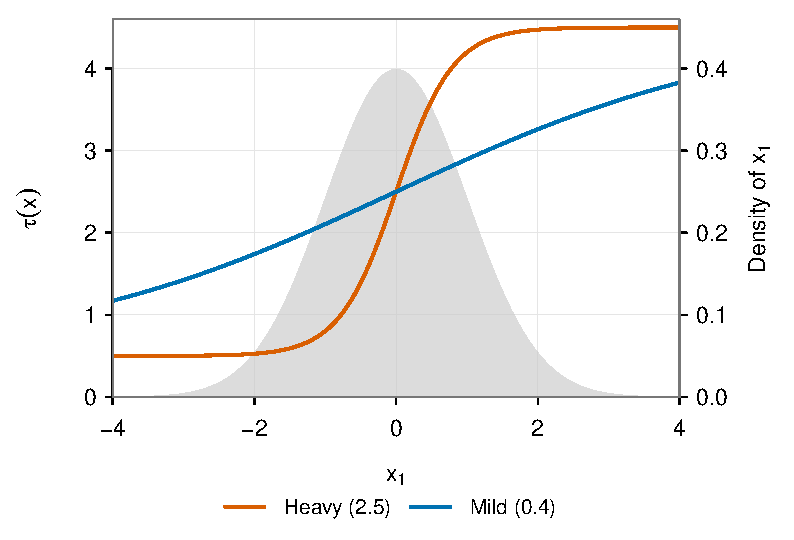
\includegraphics[width=0.65\linewidth]{pictures/plots_final/density-plot-8.3.2.pdf}
    \caption{Shape of $\tau(x)$ plotted against $x_1$ for the two saturation scenarios, with coefficients $2.5$ and $0.4$. The shaded area shows the standard normal density of $x_1$ (right axis).}
    \label{fig:saturation-density-plot}
\end{figure}

\subsubsection{Performance Measures}
For the ATE and CATE, we report root mean squared error (RMSE), empirical coverage (Cov), and the average length (Len) of the $95\%$ credible intervals. The ATE target in each replicate is the mean of the true CATEs in that sample; ATE RMSE is the square root of the mean squared estimation error across replicates. For the CATE, we first calculate the RMSE across individuals within each replicate and then average over replicates. Coverage and interval length are also averaged over replicates. With 200 independent replicates, the Monte Carlo standard error of an ATE coverage estimate near $95\%$ is about 1.5 percentage points.

We evaluate ranking using the Spearman correlation between posterior-mean CATE estimates and the true CATE. Separately, we consider the top $10\%$, $25\%$, and $50\%$ of true treatment responders. A patient is classified as a top responder only if the lower bound of their $95\%$ credible interval exceeds the true threshold for that tier. Precision and sensitivity then describe how well the models identify individuals according to their treatment benefit. This interval-based rule depends on both the point estimates and their uncertainty; Spearman correlation evaluates ordering alone. The true thresholds are available in simulation. Full results for the homogeneous treatment effect and for this threshold-based selection are reported in the Supplementary Material.

\subsection{Semi-synthetic IHDP Benchmark}
\label{subsec:ihdp_setting}
The Infant Health and Development Program (IHDP) data are a well-known semi-synthetic benchmark with real covariate data and synthetic potential outcomes under 100 different scenarios \citep{ihdp1990trial,hill2011bayesian}. The benchmark contains 747 children with 25 covariates, of which five are continuous and one is a four-level categorical variable. Our preprocessing encodes these into 27 columns. Of the children, 139 (18.6\%) are treated. All 100 data sets use the same covariates and the same treatment assignments; only the simulated potential outcomes change. Since $\tau$ is then known for every child, we can score CATE accuracy directly. The benchmark combines an exponential control mean with a linear treated mean: $\mu_0(x)=\exp\{(x+a)^\top b\}$ and $\mu_1(x)=x^\top b-\omega$, so $\tau(x)=\mu_1(x)-\mu_0(x)$. Here $a$ is the covariate offset, $b$ the coefficient vector of the response surface, and $\omega$ is chosen to give an average treatment effect of four among the treated. This is similar in spirit to the saturation settings in Subsection \ref{subsec:treatment_scenarios}, except that the non-linearity is spread over several covariates rather than concentrated in $x_1$. The benchmark and its consequences for comparing CATE estimators are discussed in more detail by \citet{curth2021really}.

The IHDP comparison is restricted to the CATE. That makes it possible to include a DR-learner, an R-learner, and an S-learner alongside \rev{SP-BART} and BCF, using ten-fold cross-validation. \rev{Bayesian logistic propensity estimates with main effects and pairwise interactions are cross-fitted within each outer training partition and reused across the fitting stages. This applies to BCF and \rev{SP-BART} as well as the DR- and R-learners, so these models use the same propensity estimates. Unlike the synthetic simulations, IHDP uses out-of-sample evaluation with inner cross-fitting; the held-out outcomes are not used to fit the propensity or outcome models.} \rev{SP-BART} uses symmetric treatment coding \rev{to give both mean outcome functions the same prior variability} and supplies this propensity estimate to its prognostic component. BCF uses binary treatment coding and adaptive treatment coding \citep{hahn2020bayesian}.

Let $\mu_0(x)$ and $\mu_1(x)$ denote the mean outcomes under control and treatment. The DR-learner estimates these two outcome regressions by cross-fitting a \texttt{SuperLearner} ensemble, using the logistic propensity estimates described above. It then builds an augmented inverse-probability-weighted pseudo-outcome \citep{kennedy2020optimal} and fits a second \texttt{SuperLearner} to that pseudo-outcome. The R-learner is a causal forest that uses cross-fitted estimates of $m(x)=\operatorname{E}(Y\mid X=x)$ from the same ensemble, together with the same propensity \citep{nie2021quasi}. The S-learner fits one \texttt{SuperLearner} outcome model to the covariates and treatment indicator and takes the contrast between the treatment arms \citep{kunzel2019metalearners}. The \texttt{SuperLearner} library used for these fits contains a generalized linear model, a penalized generalized linear model, three generalized additive models with two to four degrees of freedom, gradient boosting, and a random forest.

We evaluate the five methods using out-of-sample RMSE for the CATE, Spearman correlation with the true CATE, and the calibration slope. We also report each method's mean rank, by RMSE, within the 100 data sets. Lower RMSE and a lower mean rank are better, a higher Spearman correlation is better, and a calibration slope of one is ideal. The slope is obtained by regressing the true CATE on the estimated CATE with an intercept. For the two Bayesian methods we additionally evaluate the $95\%$ credible intervals for each individual CATE: coverage of the true $\tau_i$, how often the interval excludes zero, and the Type S error among those that do. Because exclusion rates are not comparable when methods have different coverage, we save the complete CATE posterior draws and perform a second, coverage-matched analysis, reported in the Supplementary Material. For each Bayesian model, a scale factor $c$ is chosen using the other IHDP replicates and then evaluated on the held-out replicate. The held-out response surface therefore does not determine its own scale factor, although all replicates share the same children and treatment assignments.


% =============================================================================
\newpage
\section{Results}
\label{sec:results}

\subsection{Simulation Results}

\subsubsection{\rev{Homogeneous Treatment Effect}}
\rev{In the homogeneous scenario, SP-BART and BCF perform similarly and both shrink towards homogeneity (Supplementary Table \ref{tab:hom_scenario}). The true treatment effect is constant, $\tau(x)=3$. In SP-BART, the shrinkage prior pulls the main-effect and interaction coefficients towards zero, allowing the treatment function to approach a constant. For both models, CATE RMSE decreases with sample size under linear and non-linear prognosis.}
\par\smallskip

\subsubsection{Linear Treatment Effect}

In the linear scenario, the true CATE is generated as a simple linear interaction: $\tau(x) = 1 + 2x_2x_4$. Table \ref{tab:default_scenario} shows that \rev{SP-BART} has slightly lower ATE RMSE and lower CATE RMSE, shorter interval lengths, and higher CATE coverage than BCF. The \rev{absolute} difference in CATE performance is most pronounced from $N=250$ to $N=1000$. In this range, BCF often shrinks the treatment effect back towards homogeneity because its tree prior does not represent a linear treatment surface as efficiently. As the sample size increases, BCF estimates the heterogeneity more accurately, although its RMSE for the CATE remains higher. The exact sample size at which this occurs depends on the signal-to-noise ratio. This pattern also holds when the prognostic function $\mu(x)$ is non-linear. At $N=3000$, the CATE credible intervals from \rev{SP-BART} are narrower ($0.598$) than those from BCF ($1.294$), while maintaining coverage of $98\%$.

\begin{table}[htbp]
\centering
\caption{Performance Comparison in the \textbf{Default Heterogeneous Scenario} (Linear Interaction CATE). Results are shown for models with Heterogeneous Treatment Effects, comparing Linear and Non-linear prognostic functions ($\mu$).}
\label{tab:default_scenario}
\resizebox{\textwidth}{!}{
\begin{tabular}{lr ccc ccc c ccc ccc}
\toprule
& & \multicolumn{6}{c}{\textbf{BCF}} & & \multicolumn{6}{c}{\textbf{\rev{SP-BART}}} \\
\cmidrule{3-8} \cmidrule{10-15}
$\mu(x)$ Form & $N$ & \multicolumn{3}{c}{ATE} & \multicolumn{3}{c}{CATE} & & \multicolumn{3}{c}{ATE} & \multicolumn{3}{c}{CATE} \\
\cmidrule{3-5} \cmidrule{6-8} \cmidrule{10-12} \cmidrule{13-15}
& & RMSE & Cov & Len & RMSE & Cov & Len & & RMSE & Cov & Len & RMSE & Cov & Len \\
\midrule
\multirow{6}{*}{Linear}
& 250 & 0.402 & 0.77 & 0.929 & 1.083 & 0.90 & 3.342 &  & 0.355 & 0.78 & 0.868 & 0.654 & 0.94 & 2.476 \\
& 500 & 0.213 & 0.82 & 0.586 & 0.767 & 0.92 & 2.530 &  & 0.198 & 0.83 & 0.562 & 0.390 & 0.96 & 1.652 \\
& 750 & 0.168 & 0.82 & 0.456 & 0.636 & 0.93 & 2.199 &  & 0.154 & 0.86 & 0.443 & 0.319 & 0.96 & 1.332 \\
& 1000 & 0.146 & 0.81 & 0.385 & 0.559 & 0.93 & 1.966 &  & 0.137 & 0.80 & 0.377 & 0.269 & 0.96 & 1.138 \\
& 1500 & 0.107 & 0.85 & 0.308 & 0.478 & 0.93 & 1.690 &  & 0.101 & 0.85 & 0.303 & 0.211 & 0.97 & 0.918 \\
& 3000 & 0.071 & 0.86 & 0.211 & 0.358 & 0.94 & 1.316 &  & 0.068 & 0.89 & 0.211 & 0.146 & 0.97 & 0.634 \\
\midrule
\multirow{6}{*}{Non-linear}
& 250 & 0.330 & 0.87 & 0.929 & 1.104 & 0.92 & 3.545 &  & 0.253 & 0.93 & 0.818 & 0.613 & 0.95 & 2.395 \\
& 500 & 0.192 & 0.86 & 0.575 & 0.802 & 0.92 & 2.585 &  & 0.162 & 0.90 & 0.534 & 0.372 & 0.96 & 1.590 \\
& 750 & 0.127 & 0.91 & 0.448 & 0.659 & 0.93 & 2.184 &  & 0.110 & 0.95 & 0.422 & 0.280 & 0.97 & 1.265 \\
& 1000 & 0.105 & 0.95 & 0.381 & 0.584 & 0.93 & 1.957 &  & 0.092 & 0.95 & 0.361 & 0.233 & 0.98 & 1.077 \\
& 1500 & 0.087 & 0.92 & 0.299 & 0.490 & 0.93 & 1.666 &  & 0.081 & 0.92 & 0.289 & 0.187 & 0.97 & 0.861 \\
& 3000 & 0.055 & 0.95 & 0.205 & 0.368 & 0.94 & 1.294 &  & 0.049 & 0.95 & 0.201 & 0.130 & 0.98 & 0.598 \\
\bottomrule
\end{tabular}}
\end{table}

\subsubsection{Heavy Saturation}
The comparative advantage for the point estimates shifts in favour of BCF in the heavy saturation scenario (Table \ref{tab:med_sat_scenario}). Here, the treatment effect follows a steep sigmoid curve and is non-linear. The RMSEs are similar at $N=250$. BCF has lower CATE RMSE and better coverage at every sample size because the tree-based treatment function can capture the steep curve by splitting on $x_1$. As $N$ increases, the posterior of \rev{SP-BART} concentrates around a biased linear approximation, causing its credible intervals to shrink and coverage to decrease. BCF's advantage under heavy saturation is on the CATE magnitudes. On ranking the order reverses: \rev{SP-BART} has higher Spearman correlation in every cell (Table \ref{tab:simulation_spearman}). It also recovers more of the true top decile at higher precision under the interval-based selection rule (Section \ref{subsec:ranking_supp}). When the treatment function is monotone, the linear approximation therefore hurts the estimated sizes more than the ordering of patients.

\begin{table}[htbp]
\centering
\caption{Performance Comparison in the \textbf{Heavy Saturation Scenario} (Non-linear Sigmoid CATE). Results are shown for models with Heterogeneous Treatment Effects, comparing Linear and Non-linear prognostic functions ($\mu(x)$).}
\label{tab:med_sat_scenario}
\resizebox{\textwidth}{!}{
\begin{tabular}{lr ccc ccc c ccc ccc}
\toprule
& & \multicolumn{6}{c}{\textbf{BCF}} & & \multicolumn{6}{c}{\textbf{\rev{SP-BART}}} \\
\cmidrule{3-8} \cmidrule{10-15}
$\mu(x)$ Form & $N$ & \multicolumn{3}{c}{ATE} & \multicolumn{3}{c}{CATE} & & \multicolumn{3}{c}{ATE} & \multicolumn{3}{c}{CATE} \\
\cmidrule{3-5} \cmidrule{6-8} \cmidrule{10-12} \cmidrule{13-15}
& & RMSE & Cov & Len & RMSE & Cov & Len & & RMSE & Cov & Len & RMSE & Cov & Len \\
\midrule
\multirow{6}{*}{Linear}
& 250 & 0.349 & 0.79 & 0.867 & 0.701 & 0.94 & 2.607 &  & 0.354 & 0.81 & 0.878 & 0.755 & 0.88 & 2.353 \\
& 500 & 0.205 & 0.82 & 0.563 & 0.499 & 0.94 & 1.906 &  & 0.200 & 0.83 & 0.567 & 0.563 & 0.83 & 1.553 \\
& 750 & 0.159 & 0.85 & 0.444 & 0.421 & 0.94 & 1.595 &  & 0.160 & 0.86 & 0.448 & 0.525 & 0.76 & 1.260 \\
& 1000 & 0.142 & 0.81 & 0.378 & 0.369 & 0.94 & 1.406 &  & 0.141 & 0.81 & 0.382 & 0.499 & 0.70 & 1.073 \\
& 1500 & 0.104 & 0.84 & 0.303 & 0.315 & 0.94 & 1.178 &  & 0.103 & 0.84 & 0.307 & 0.473 & 0.60 & 0.867 \\
& 3000 & 0.070 & 0.88 & 0.210 & 0.238 & 0.93 & 0.872 &  & 0.068 & 0.91 & 0.213 & 0.452 & 0.42 & 0.603 \\
\midrule
\multirow{6}{*}{Non-linear}
& 250 & 0.290 & 0.86 & 0.851 & 0.704 & 0.96 & 2.723 &  & 0.252 & 0.91 & 0.828 & 0.717 & 0.90 & 2.265 \\
& 500 & 0.177 & 0.88 & 0.544 & 0.505 & 0.96 & 1.907 &  & 0.166 & 0.91 & 0.539 & 0.554 & 0.83 & 1.497 \\
& 750 & 0.116 & 0.94 & 0.431 & 0.401 & 0.96 & 1.573 &  & 0.110 & 0.95 & 0.428 & 0.504 & 0.76 & 1.189 \\
& 1000 & 0.097 & 0.95 & 0.367 & 0.348 & 0.96 & 1.386 &  & 0.091 & 0.96 & 0.366 & 0.480 & 0.70 & 1.018 \\
& 1500 & 0.084 & 0.91 & 0.293 & 0.294 & 0.96 & 1.144 &  & 0.082 & 0.92 & 0.294 & 0.464 & 0.58 & 0.813 \\
& 3000 & 0.052 & 0.94 & 0.202 & 0.213 & 0.95 & 0.841 &  & 0.051 & 0.95 & 0.204 & 0.447 & 0.39 & 0.571 \\
\bottomrule
\end{tabular}}
\end{table}

\subsubsection{Mild Saturation}

The mild saturation scenario provides a less severe departure from linearity. Table \ref{tab:mild_ate_cate} presents the RMSE, empirical coverage, and average length of the 95\% credible intervals in this setting. When the treatment effect saturates slowly as $x_1$ increases, it can be approximated by a linear gradient. From $N=500$, \rev{SP-BART} has lower CATE RMSE than BCF, with CATE coverage close to or above nominal. Its CATE intervals become shorter from $N=500$, while at $N=250$ BCF has slightly lower CATE RMSE and shorter intervals.

ATE coverage is less satisfactory than CATE coverage in the structurally aligned settings. With a linear prognostic function, the nominal $95\%$ ATE intervals undercover for both models across the scenarios. The favourable CATE results therefore do not imply well-calibrated inference for the ATE. \rev{Under linear prognosis, both models have positive ATE bias. In the linear treatment-effect scenario, mean ATE errors decrease from $0.251$ at $N=250$ to $0.046$ at $N=3000$ for \rev{SP-BART}, and from $0.286$ to $0.050$ for BCF. The positive ATE bias suggests that both models do not fully adjust for selection in this setting.}


\begin{table}[H]
\centering
\caption{Performance Metrics: Mild Saturation Scenario. Evaluation of the Average Treatment Effect (ATE) and Conditional Average Treatment Effect (CATE) across varying sample sizes ($N$) and functional forms of the prognostic score ($\mu(x)$).}
\label{tab:mild_ate_cate}
\resizebox{\textwidth}{!}{
\begin{tabular}{lr ccc ccc c ccc ccc}
\toprule
& & \multicolumn{6}{c}{\textbf{ BCF}} & & \multicolumn{6}{c}{\textbf{\rev{SP-BART}}} \\
\cmidrule{3-8} \cmidrule{10-15}
$\mu(x)$ Form & $N$ & \multicolumn{3}{c}{ATE} & \multicolumn{3}{c}{CATE} & & \multicolumn{3}{c}{ATE} & \multicolumn{3}{c}{CATE} \\
\cmidrule{3-5} \cmidrule{6-8} \cmidrule{10-12} \cmidrule{13-15}
& & RMSE & Cov & Len & RMSE & Cov & Len & & RMSE & Cov & Len & RMSE & Cov & Len \\
\midrule
\multirow{6}{*}{Linear}
& 250 & 0.326 & 0.80 & 0.854 & 0.554 & 0.94 & 2.118 &  & 0.350 & 0.80 & 0.862 & 0.611 & 0.94 & 2.294 \\
& 500 & 0.197 & 0.83 & 0.559 & 0.406 & 0.95 & 1.565 &  & 0.197 & 0.83 & 0.559 & 0.359 & 0.96 & 1.524 \\
& 750 & 0.153 & 0.86 & 0.443 & 0.346 & 0.95 & 1.313 &  & 0.153 & 0.86 & 0.441 & 0.296 & 0.96 & 1.232 \\
& 1000 & 0.138 & 0.82 & 0.378 & 0.312 & 0.94 & 1.156 &  & 0.137 & 0.81 & 0.376 & 0.247 & 0.96 & 1.050 \\
& 1500 & 0.102 & 0.87 & 0.303 & 0.265 & 0.95 & 0.978 &  & 0.101 & 0.86 & 0.303 & 0.193 & 0.97 & 0.846 \\
& 3000 & 0.069 & 0.89 & 0.210 & 0.201 & 0.94 & 0.726 &  & 0.068 & 0.90 & 0.210 & 0.136 & 0.96 & 0.582 \\
\midrule
\multirow{6}{*}{Non-linear}
& 250 & 0.250 & 0.93 & 0.831 & 0.557 & 0.96 & 2.075 &  & 0.250 & 0.92 & 0.817 & 0.564 & 0.95 & 2.222 \\
& 500 & 0.161 & 0.91 & 0.538 & 0.418 & 0.94 & 1.474 &  & 0.161 & 0.91 & 0.530 & 0.343 & 0.96 & 1.466 \\
& 750 & 0.110 & 0.94 & 0.427 & 0.330 & 0.96 & 1.244 &  & 0.108 & 0.96 & 0.421 & 0.255 & 0.97 & 1.164 \\
& 1000 & 0.093 & 0.95 & 0.364 & 0.296 & 0.95 & 1.118 &  & 0.091 & 0.95 & 0.360 & 0.211 & 0.98 & 0.994 \\
& 1500 & 0.082 & 0.93 & 0.292 & 0.248 & 0.96 & 0.942 &  & 0.080 & 0.91 & 0.289 & 0.170 & 0.97 & 0.790 \\
& 3000 & 0.051 & 0.95 & 0.202 & 0.176 & 0.97 & 0.696 &  & 0.049 & 0.96 & 0.200 & 0.118 & 0.98 & 0.550 \\
\bottomrule
\end{tabular}}
\end{table}

\subsubsection{Ranking Performance}

Table \ref{tab:simulation_spearman} reports Spearman correlations with the true CATE. \rev{SP-BART} has higher mean correlation in every heterogeneous simulation cell. In the linear scenario, correlations range from $0.960$ to $0.998$, compared with $0.889$ to $0.990$ for BCF. Under heavy saturation they range from $0.924$ to $0.997$, compared with $0.888$ to $0.985$ for BCF. Thus, the linear approximation can preserve the ordering of patients even when it biases the CATE magnitudes. Ranking is more difficult for both methods under mild saturation, where the treatment effect varies less.

The interval-based selection results in the Supplementary Material (Section \ref{subsec:ranking_supp}) provide a related comparison. Under heavy saturation \rev{SP-BART} recovers more of the true top decile than BCF with higher precision, despite its poor coverage in this scenario. Results are more mixed at the $25\%$ and $50\%$ thresholds. These selection results also depend on interval width and calibration, and should be read alongside the Spearman correlations. \rev{The full ranking tables, including the broader thresholds, are in the Supplementary Material.}

\begin{table}[htbp]
\centering\small
\caption{Spearman correlation between posterior-mean CATE estimates and the true CATE in simulation. Values are means (Monte Carlo standard errors) over 200 replicates. Spearman correlation is undefined for the homogeneous treatment effect.}
\label{tab:simulation_spearman}
\resizebox{\textwidth}{!}{%
\begin{tabular}{llcccc}
\toprule
& & \multicolumn{2}{c}{Linear $\mu(x)$} & \multicolumn{2}{c}{Non-linear $\mu(x)$} \\
\cmidrule(lr){3-4}\cmidrule(lr){5-6}
Scenario & $N$ & BCF & \rev{SP-BART} & BCF & \rev{SP-BART} \\
\midrule
\multirow{6}{*}{Linear} & 250 & 0.891 (0.0031) & 0.960 (0.0021) & 0.889 (0.0034) & 0.960 (0.0026) \\
 & 500 & 0.947 (0.0013) & 0.986 (0.0006) & 0.945 (0.0015) & 0.985 (0.0008) \\
 & 750 & 0.964 (0.0009) & 0.990 (0.0005) & 0.964 (0.0010) & 0.992 (0.0004) \\
 & 1000 & 0.973 (0.0007) & 0.993 (0.0004) & 0.971 (0.0008) & 0.994 (0.0003) \\
 & 1500 & 0.980 (0.0005) & 0.996 (0.0002) & 0.981 (0.0005) & 0.996 (0.0002) \\
 & 3000 & 0.989 (0.0002) & 0.998 (0.0001) & 0.990 (0.0003) & 0.998 (0.0001) \\
\midrule
\multirow{6}{*}{Heavy saturation} & 250 & 0.888 (0.0039) & 0.924 (0.0051) & 0.893 (0.0038) & 0.932 (0.0046) \\
 & 500 & 0.932 (0.0022) & 0.975 (0.0013) & 0.936 (0.0020) & 0.975 (0.0015) \\
 & 750 & 0.949 (0.0017) & 0.983 (0.0009) & 0.954 (0.0015) & 0.985 (0.0009) \\
 & 1000 & 0.959 (0.0013) & 0.988 (0.0006) & 0.962 (0.0011) & 0.989 (0.0006) \\
 & 1500 & 0.967 (0.0009) & 0.992 (0.0004) & 0.973 (0.0008) & 0.993 (0.0004) \\
 & 3000 & 0.980 (0.0006) & 0.996 (0.0002) & 0.985 (0.0005) & 0.997 (0.0002) \\
\midrule
\multirow{6}{*}{Mild saturation} & 250 & 0.433 (0.0164) & 0.507 (0.0204) & 0.422 (0.0159) & 0.611 (0.0175) \\
 & 500 & 0.610 (0.0128) & 0.762 (0.0111) & 0.575 (0.0148) & 0.790 (0.0105) \\
 & 750 & 0.700 (0.0113) & 0.819 (0.0093) & 0.713 (0.0119) & 0.860 (0.0073) \\
 & 1000 & 0.755 (0.0098) & 0.866 (0.0078) & 0.763 (0.0100) & 0.900 (0.0048) \\
 & 1500 & 0.824 (0.0069) & 0.911 (0.0046) & 0.854 (0.0058) & 0.937 (0.0032) \\
 & 3000 & 0.902 (0.0039) & 0.959 (0.0021) & 0.930 (0.0027) & 0.967 (0.0016) \\
\bottomrule
\end{tabular}}
\end{table}

In a separate simulation of the linear interaction treatment effect, we also investigated residualising the treatment indicator. This variant increased the CATE RMSE under both prognostic forms (Supplementary Section \ref{subsec:ortho_supp}).

Overall, BCF performs better on CATE magnitudes when the treatment effect cannot be represented by main effects and pairwise interactions. When subgroup heterogeneity is represented well by these terms, \rev{SP-BART} estimates the CATE more efficiently in these simulations.

\subsection{IHDP Results}
\label{subsec:ihdp}

The IHDP benchmark is a challenging setting for \rev{SP-BART} because the true treatment effect is the difference between linear and exponential mean outcome surfaces. Despite this structural mismatch, the model approximates the CATE surface and performs on par with BCF (Table \ref{tab:ihdp_primary}). BCF has a slightly lower mean RMSE ($1.720$ versus $1.739$ for \rev{SP-BART}), a lower median RMSE, and the lower RMSE in 75 of the 100 data sets. BCF also has the lower mean rank and a calibration slope closer to one, as well as a higher mean Spearman correlation ($0.892$ versus $0.879$).

Of the five implementations, the two Bayesian methods have the lowest mean RMSE and the lowest mean rank, and the two highest mean Spearman correlations. Calibration is more mixed: BCF is closest to a slope of one. Both models use the same BART prior for the prognostic function and differ on the priors chosen to model the treatment contrast. We observe that the pairwise interactions still approximate the non-linear treatment function over the observed covariate support, because they allow the effect of one covariate to depend on another.

The signal-stratified results in Table \ref{tab:ihdp_signal_bands} reverse the ordering of the two Bayesian methods. BCF has the lower RMSE in 24 of the 25 data sets in the weakest quartile, whereas \rev{SP-BART} has the lower RMSE in 16 of the 25 data sets in the strongest quartile. This matches the simulations. A linear treatment function uses a structured signal more efficiently, while BCF shrinks more towards a homogeneity. When the treatment effect varies less, as in the weakest quartile, the extra shrinkage helps. When the CATE signal is pronounced, \rev{SP-BART} fares better. The quartiles also differ in the scale and shape of $\tau$, so signal strength is probably not the only reason. What the split does show is that the two Bayesian models do not rank the same way in every IHDP scenario.


\begin{table}[H]
\centering\footnotesize
\caption{IHDP benchmark. Results over 100 replicates using 10-fold out-of-sample predictions. Values are mean (standard error) unless stated. RMSE is for the CATE. The mean rank is the average rank by RMSE across the 100 data sets.}
\label{tab:ihdp_primary}
\resizebox{\textwidth}{!}{%
\begin{tabular}{lccccc}
\toprule
Method & RMSE & median RMSE & Spearman & Calib.\ slope & mean rank\\
\midrule
\textbf{\rev{SP-BART}} & 1.739 (0.242) & 0.957 & 0.879 (0.015) & 0.808 (0.022) & 2.08\\
BCF & \textbf{1.720} (0.269) & \textbf{0.819} & \textbf{0.892} (0.018) & \textbf{0.928} (0.022) & \textbf{1.36}\\
DR-learner & 2.343 (0.250) & 1.618 & 0.716 (0.029) & 0.786 (0.033) & 3.88\\
S-learner & 3.109 (0.453) & 1.545 & 0.817 (0.023) & 1.822 (0.085) & 3.41\\
R-learner & 4.212 (0.635) & 1.912 & 0.726 (0.017) & 1.715 (0.058) & 4.27\\
\bottomrule
\end{tabular}
}
\end{table}

\begin{table}[H]
\centering\small
\caption{Performance of the two Bayesian methods by the amount of treatment
effect signal present, measured by quartiles of $\operatorname{sd}(\tau)$ across
the 100 data sets. $\Delta$ is the difference in RMSE (for the CATE) between \rev{SP-BART} and BCF, so a negative value favours \rev{SP-BART}.}
\label{tab:ihdp_signal_bands}
\begin{tabular}{ccrrrr}
\toprule
Quartile & range of $\operatorname{sd}(\tau)$ & data sets & mean $\Delta$ & median $\Delta$ & \rev{SP-BART}\ wins\\
\midrule
1 (weakest) & 0.03--1.08 & 25 & 0.139 & 0.135 & 1/25\\
2 & 1.15--2.54 & 25 & 0.126 & 0.123 & 2/25\\
3 & 2.57--5.55 & 25 & 0.149 & 0.162 & 6/25\\
4 (strongest) & 5.67--43.22 & 25 & $-0.338$ & $-0.228$ & 16/25\\
\bottomrule
\end{tabular}
\end{table}

\subsection{Individual CATE Posteriors on IHDP}
\label{subsec:ihdp_posterior}

In addition to the point estimates, we also evaluate whether the models correctly predict harm or benefit, and how they quantify uncertainty. The IHDP outcomes are synthetic, so we can check the sign of each posterior and whether the interval covers the true effect. We report how often the $95\%$ interval excludes zero, and the Type S error among those that do (Table \ref{tab:ihdp_posterior}). The same quantities are split by quartiles of signal strength of the treatment effect in Table \ref{tab:ihdp_posterior_bands}.

The main difference is the length of the credible intervals. \rev{SP-BART} has wider intervals, while the shorter intervals of BCF exclude zero more often. This extra confidence comes at a price. BCF undercovers more than \rev{SP-BART} in every signal quartile, and its Type S rate is slightly higher overall, although not in the strongest quartile (Table \ref{tab:ihdp_posterior_bands}). The AUC for $P(\tau_i>0)$ as a classifier of the sign of $\tau_i$, i.e. how well the model can discriminate between a true negative and true positive effect is higher for \rev{SP-BART}. Coverage is still below the nominal $95\%$ for both methods except in the weakest quartile.

The exclusion rates before calibration in Table~\ref{tab:ihdp_posterior} are therefore not a fair comparison of how often each model can detect a non-zero effect. The \rev{SP-BART} intervals cover $93.0\%$ of the true $\tau_i$, against $91.4\%$ for BCF. We use the posterior draws to rescale each model's intervals towards a common empirical coverage target of $95\%$. The amount of adjustment was chosen from the remaining 99 data sets and then applied to the held-out one, so the same replicate is not used both to set the interval and to score it. The Supplementary Material (Section~\ref{subsec:ihdp_matched_supp}, Table~\ref{tab:ihdp_posterior_matched}) reports the result. BCF's intervals have to be expanded the most ($c=1.186$), while \rev{SP-BART} needs $c=1.105$. At approximately matched coverage, the exclusion rates are close: $87.6\%$ of children for \rev{SP-BART} and $87.8\%$ for BCF (paired difference $-0.0015$, $95\%$ CI $[-0.0101,0.0072]$). The higher exclusion rate of BCF before calibration therefore becomes much smaller at comparable empirical coverage.

\begin{table}[H]
\centering\footnotesize
\caption{Individual CATE posteriors on IHDP (100 replicates, 10-fold out-of-sample,
$95\%$ credible intervals). Values are mean (standard error) over the 100 data sets, except AUC, which is averaged where both true effect signs occur.
``Excludes $0$'' is the fraction of children whose interval excludes zero.
``Sign correct'' and ``Type S'' are conditional on that. Coverage is of the true $\tau_i$
(nominal $0.95$). AUC is for $P(\tau_i>0)$ as a classifier of $\operatorname{sign}(\tau_i)$.}
\label{tab:ihdp_posterior}
\resizebox{\textwidth}{!}{%
\begin{tabular}{lcccccc}
\toprule
Method & excludes $0$ & sign correct & Type S & coverage & width & AUC $P(\tau>0)$\\
\midrule
\textbf{\rev{SP-BART}} & 0.890 (0.007) & \textbf{0.998} (0.000) & \textbf{0.002} (0.000) & \textbf{0.930} (0.005) & 5.04 (0.55) & \textbf{0.992} (0.001)\\
BCF & \textbf{0.897} (0.009) & 0.997 (0.000) & 0.003 (0.000) & 0.914 (0.005) & 4.55 (0.64) & 0.976 (0.008)\\
\bottomrule
\end{tabular}}
\end{table}

\begin{table}[H]
\centering\small
\caption{Coverage of the true $\tau_i$ and Type S error rate by quartile of
$\operatorname{sd}(\tau)$, using the same quartiles as Table
\ref{tab:ihdp_signal_bands}. Nominal coverage is $0.95$.}
\label{tab:ihdp_posterior_bands}
\begin{tabular}{lcccc}
\toprule
& \multicolumn{2}{c}{Coverage} & \multicolumn{2}{c}{Type S (\%)}\\
\cmidrule(lr){2-3}\cmidrule(lr){4-5}
Quartile of $\operatorname{sd}(\tau)$ & BCF & \rev{SP-BART} & BCF & \rev{SP-BART}\\
\midrule
1 (weakest) & 0.961 & \textbf{0.963} & 0.05 & \textbf{0.02}\\
2 & 0.928 & \textbf{0.944} & 0.38 & \textbf{0.11}\\
3 & 0.898 & \textbf{0.932} & 0.29 & \textbf{0.17}\\
4 (strongest) & 0.870 & \textbf{0.880} & \textbf{0.41} & 0.47\\
\bottomrule
\end{tabular}
\end{table}

% =============================================================================
\section{Applied Example: The CANVAS Program}
\label{subsec:applied_example}
We applied \rev{SP-BART} to individual participant data from the CANVAS Program. We consider two randomized, double-blind, placebo-controlled trials, CANVAS (NCT01032629) and CANVAS-R (NCT01989754), designed to evaluate the cardiovascular and renal effects of the SGLT2 inhibitor canagliflozin in patients with type 2 diabetes at high cardiovascular risk \citep{neal2013rationale, neal2017rationale}. Access to this trial data was granted under the Yale University Open Data Access (YODA) Project (Access Request Number: \textbf{2025-0684}). The primary continuous outcome measure for this analysis is the change in HbA1c from baseline to the 52-week follow-up. HbA1c reflects average blood glucose levels over the past months and is therefore a key marker of the glucose-lowering effect of SGLT2 inhibitors. This treatment window has also been used to evaluate glycaemic efficacy in earlier canagliflozin research \citep{cefalu2013efficacy}.

We compare canagliflozin with placebo. To capture potential drivers of treatment effect heterogeneity, we selected a set of baseline participant characteristics, including baseline HbA1c, age, urinary albumin-to-creatinine ratio, eGFR, systolic blood pressure, history of cerebrovascular disease, diabetes duration, and sex. We also included body mass index, recorded race, history of heart failure, and baseline use of insulin, metformin, GLP-1 receptor agonists, and agents acting on the renin--angiotensin system. The full covariate list and coding are given in Supplementary Section \ref{SEC:supplement_canvas}. \rev{We used complete cases for the 52-week HbA1c change, treatment assignment, and selected baseline covariates; missing values were not imputed. \rev{SP-BART} uses symmetric treatment coding to give both mean outcome functions the same prior variability, while BCF uses adaptive treatment coding. Both models include the treatment proportion in the full CANVAS-R training pool as the same constant propensity score in the prognostic component.} The Shapley decomposition and coefficient posteriors are presented below.

\subsection{Results and Interpretability}
\label{subsec:oos_performance_summary}

We trained both models on the CANVAS-R analytic sample and evaluated them in the CANVAS analytic sample. In the smaller training samples, both models shrink the estimated treatment effects towards homogeneity, more so for BCF (Supplementary Section \ref{SEC:supplement_canvas}). At the full CANVAS-R sample, the correlation between their out-of-sample CATE predictions is $r=0.843$; at $N=4000$ it is $0.813$ (Table \ref{tab:model_metrics}). The models rank patients similarly by predicted benefit, while \rev{SP-BART} has lower out-of-sample RMSE for HbA1c change at every training size. When their rankings are similar, \rev{SP-BART} also gives direct parameter-level inference on the treatment-effect modifiers.

RACE, considered jointly, has the largest grouped Shapley contribution, followed by baseline HbA1c and age; these contributions arise mainly through main effects. \rev{Figure \ref{fig:shapley_contribution} shows their contributions across individuals.} Higher baseline HbA1c generally contributes to a larger treatment-related reduction in HbA1c, while older age contributes to a smaller reduction.

\begin{figure}[p]
    \centering
    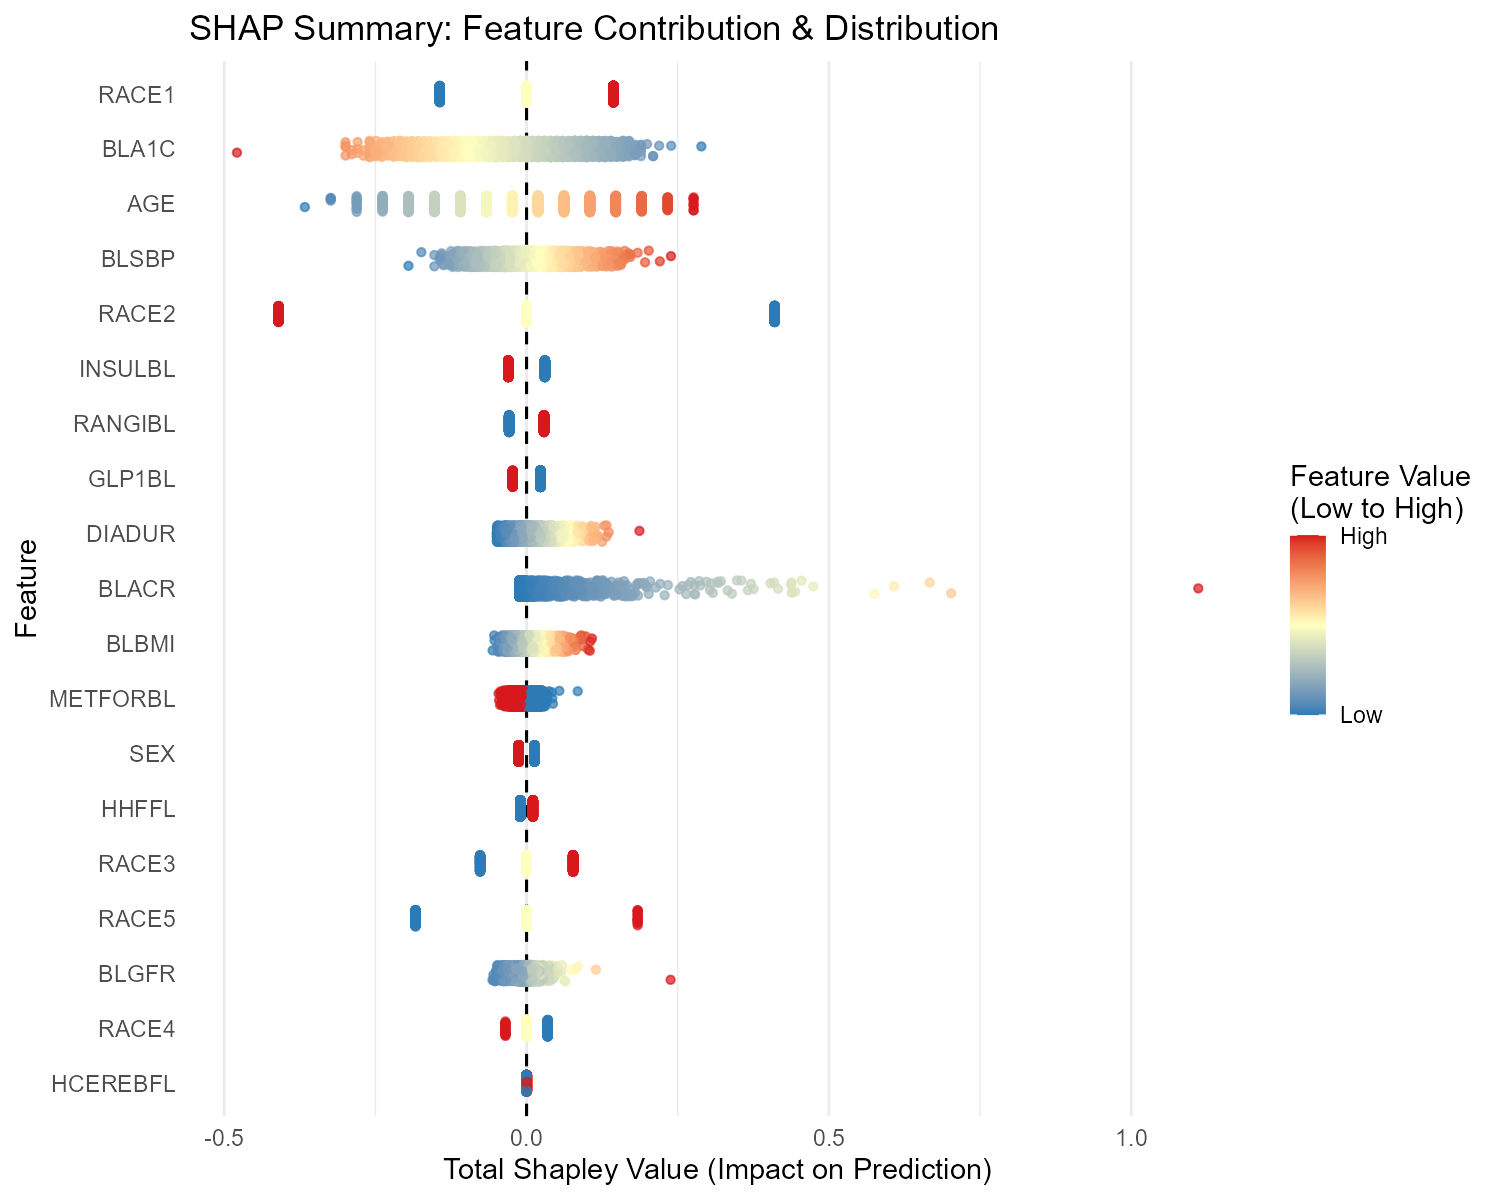
\includegraphics[width=\textwidth]{shapley_distribution.png}
    \caption{Individual Shapley summaries for the predicted CATE in CANVAS-R. Each point adds the posterior medians of one individual's main-effect and interaction contributions. Colour indicates the covariate value, from low (blue) to high (red). Negative contributions indicate a larger HbA1c reduction. RACE1--RACE5 are contrast columns of one categorical covariate. The spread describes variation between individuals. Abbreviations are defined in Supplementary Table \ref{tab:canvas_covariates}.}
    \label{fig:shapley_contribution}
\end{figure}

Simultaneous $95\%$ posterior intervals for the treatment-effect contrasts of baseline HbA1c, age, and RACE exclude zero. \rev{The RACE contrast indicates a larger estimated treatment-related HbA1c reduction for Black or African American than for White participants (Supplementary Figure \ref{fig:canvas_full_contrasts}).} These contrasts include interactions and are averaged over the empirical distribution of the other covariates (Supplementary Section \ref{subsec:applied_interpretability}). BCF provides posterior CATEs but does not give the same direct inference about individual modifiers. The clinical interpretation of the race-related pattern remains uncertain. \rev{An earlier pooled analysis, including CANVAS sub-studies, found HbA1c reductions across racial groups, but the studies were not powered to assess racial differences \citep{gavin2015racial}. A CANVAS Program analysis compared Asian and White participants for cardiovascular and renal outcomes \citep{chen2024ethnic}; those outcomes do not directly establish the race-related pattern in 52-week HbA1c change found here.}

\subsection{Posterior Distributions of the Main Effects}
\label{sec:posterior_behaviour}
Figure \ref{fig:posterior_HBA1C} shows the posteriors of the main-effect coefficients for baseline HbA1c and age. Their means are $-0.094$ and $0.090$, with pointwise $95\%$ credible intervals $[-0.145,-0.044]$ and $[0.033,0.147]$, respectively, on the fitted model scale. With the other encoded covariates held at zero, higher baseline HbA1c is associated with a larger treatment-related reduction in HbA1c, while older age is associated with a smaller reduction. These are main-effect coefficients; the full treatment-effect contrasts also include interactions.

\begin{figure}[H]
    \centering
    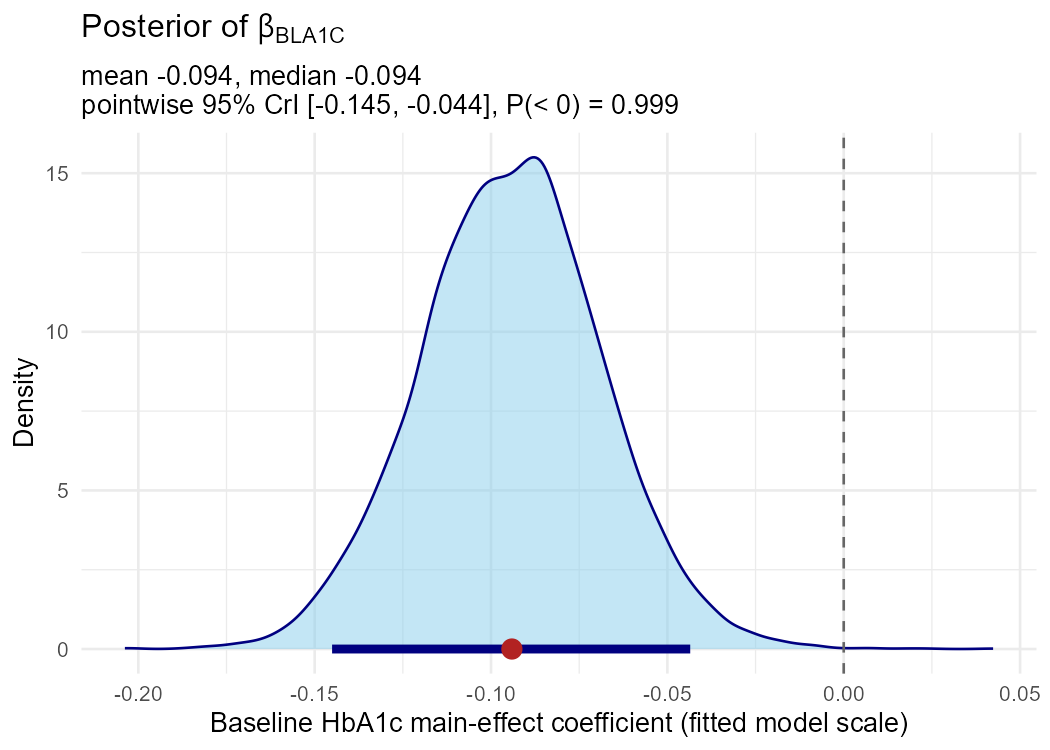
\includegraphics[width=0.60\linewidth]{posterior_BLA1C_beta (1).png}
    \par\medskip
    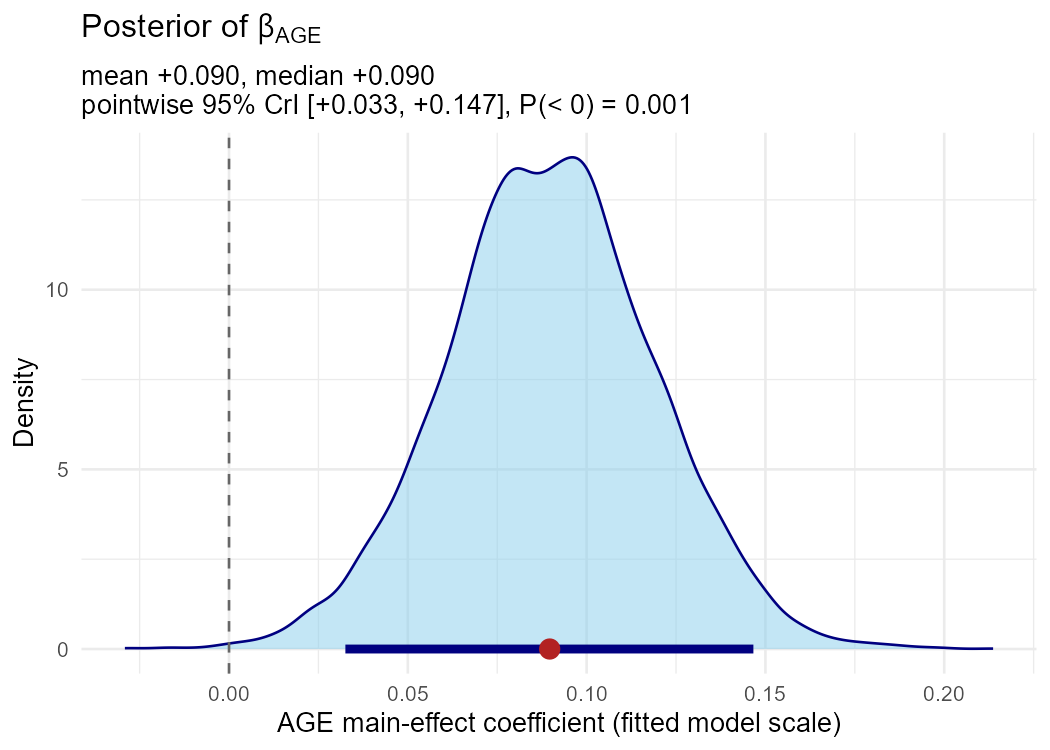
\includegraphics[width=0.60\linewidth]{posterior_AGE_beta (1).png}
    \caption{Posterior distributions of the main-effect coefficients for baseline HbA1c (upper panel) and age (lower panel). Both pointwise $95\%$ credible intervals exclude zero.}
    \label{fig:posterior_HBA1C}
    \label{fig:posterior_AGE}
\end{figure}
\FloatBarrier

\section{Code and Data Availability}
\label{sec:availability}
The simulation, IHDP, and application analysis scripts are available at \rev{\url{https://github.com/HYHBalci/spbart-paper}}. The model implementation for general use is available in \rev{\texttt{spbart}, based on \texttt{stochtree}, at \url{https://github.com/HYHBalci/spbart}}. The analysis repository includes data-generating code, model fitting, and evaluation scripts. CANVAS participant data are available through the Yale University Open Data Access Project under \href{https://yoda.yale.edu/data-request/2025-0684/}{request 2025-0684}, subject to its access requirements.

\section{Discussion}
\label{sec:discussion}
We presented \rev{SP-BART, which} places a flexible BART prior on the prognostic function and a sparse linear model, with main effects and pairwise interactions, on the treatment effect. The global--local shrinkage prior makes it possible to search a large interaction space. Shapley values then summarize how each covariate contributes to the CATE. The model also provides conditional mean potential-outcome predictions, besides CATE estimation.

The results return to the four questions from the Introduction: who benefits, why benefit varies, how certain that benefit is, and what would happen under either treatment.

The simulations describe the trade-off that this structure creates. When the treatment effect is linear, or close enough to a linear gradient, \rev{SP-BART} generally has lower CATE RMSE and, at larger sample sizes, tighter credible intervals than BCF. When the treatment function is more strongly non-linear, BCF has lower RMSE and better coverage. Spearman ranking favours \rev{SP-BART} in all heterogeneous simulation settings. Under monotone saturation it is also generally the more sensitive and the more precise of the two at the sharpest interval-based threshold. ATE coverage is less satisfactory under linear prognosis: both models' nominal $95\%$ ATE intervals fall below nominal coverage, alongside positive ATE bias. Residual bias under targeted selection may contribute, although these results do not identify its source.

We primarily compare with BCF because both models use a BART prognostic component, allowing us to examine the effect of modelling the treatment contrast parametrically or with a second forest. IHDP provides a broader comparison with the DR-, S-, and R-learners.

On IHDP the true treatment effect is the difference between linear and exponential mean outcome surfaces, so it does not lie in the linear-plus-interactions span of our model. Even so, the approximation is close enough that \rev{SP-BART} performs on par with BCF. The two Bayesian methods have the first and second lowest mean RMSE and mean rank, they have the two highest mean Spearman correlations with the true CATE, and both outperform the implementations of the frequentist machine learners considered here (the DR-learner, the S-learner, and the R-learner) on these metrics. Comparing the two Bayesian methods on individual inference, BCF excludes zero from the individual intervals more often, while \rev{SP-BART} has wider intervals, better coverage of the true $\tau_i$, and fewer Type S errors overall. Neither method attains the nominal $95\%$ coverage except in the weakest quartile. After calibrating the intervals towards the same empirical coverage, \rev{SP-BART} and BCF have very similar exclusion rates. We can do this calibration because the true effects are known in IHDP.

In CANVAS, the two models rank patients similarly, while \rev{SP-BART} has lower out-of-sample outcome prediction error. Its grouped Shapley decomposition places RACE, baseline HbA1c, and age among the largest contributors to treatment-effect heterogeneity, mainly through main effects. The corresponding full CATE contrasts have simultaneous $95\%$ posterior intervals that exclude zero. \rev{SP-BART} provides these contrasts directly; BCF's CATE posterior does not give the same parameter-level inference.

The gain in efficiency still comes with a structural limitation: non-linearity in the treatment function cannot always be represented by main effects and pairwise interactions. The IHDP results qualify this limitation, since a smooth non-linear treatment function can still be approximated using the main and interaction effects. The heavy saturation results show where this approximation starts to break down.

Including more covariates and their pairwise interactions increases the number of coefficients and the computation required for fitting. The propensity score enters the prognostic function as an additional covariate, while the outcome model provides the treatment-effect estimates.

\subsection{Guidance for Practice}
In practice, \rev{SP-BART} is the more natural choice when treatment effect heterogeneity is expected to be represented well by main effects and pairwise interactions, and when direct inference on effect modifiers or prediction of both potential outcomes is required. BCF is safer when strong non-linearity in the treatment function is plausible, or when simulations indicate that the linear treatment function loses coverage.

In real data, where the CATE is not known, out-of-sample outcome prediction can help to decide between the two models. In a randomized validation sample, patients can also be grouped by predicted benefit. Comparing the observed treatment--control differences with the predicted mean treatment effects in these groups then assesses calibration at group level. When performance is similar, we prefer \rev{SP-BART}, because it provides more interpretability at the parameter level. We also advise evaluating the agreement between the CATE rankings of the two models, because this assesses the robustness of the ranking with respect to model choice. Strong disagreement between the models calls for further model checking rather than favouring either model by itself.

\subsection{Future Directions}
Rather than estimating a sparse signal with a treatment function, future work might directly classify whether individuals do or do not benefit from a treatment. Recent work by \cite{muller2025data} and \cite{cheng2025chiseling} provides frameworks for identifying subgroups with treatment benefit while controlling specified error rates under their respective assumptions. Given that our model can capture the prognostic function, the remaining partial residuals could be used to classify patients into subgroups without explicitly modelling the treatment effect function. Furthermore, \cite{chen2026comparing} present a global test for heterogeneity based on whether score residuals are associated with the covariates. A formulation that uses a BART prior for the prognostic function could extend this test. The same backfitting scheme also extends to a Student-$t$ working likelihood for continuous outcomes with heavy tails, and to a probit model for binary outcomes; both variants are implemented, but we do not evaluate them here. When the coefficient space grows, prior specifications that link shrinkage across main and interaction effects may improve estimation \citep{van2024linked}. Future work could also examine how \rev{more flexible propensity-score models} account for the targeted-selection mechanism.

\section{Conclusion}
\label{sec:conclusion}
In summary, we provide \rev{SP-BART}, a semi-parametric Bayesian model for individualized treatment effect estimation in observational studies and randomized trials. It combines a non-parametric prognostic component with a sparse linear treatment effect component, providing direct parameter inference and patient-specific predictions of conditional mean potential outcomes. In the simulations and IHDP, the interaction basis is efficient under linearity and also approximates smooth non-linearity over the observed covariate support. On IHDP, both Bayesian methods outperform the DR-learner, S-learner, and R-learner implementations considered here in mean CATE RMSE and ranking. In CANVAS, the two Bayesian models rank patients similarly, while \rev{SP-BART} provides evidence of effect modification by baseline HbA1c, age, and RACE. When main effects and pairwise interactions are a plausible description or approximation of the heterogeneity, and when inference on the modifiers themselves is of interest, \rev{SP-BART} is the more natural choice. If the two models perform similarly, we prefer \rev{SP-BART} for its interpretability. BCF remains the safer default if the treatment effect is very non-linear in a way that this basis cannot represent.



\bibliographystyle{apalike}
\bibliography{references-8.3.5}

\end{document}
